\documentclass[11pt,a4paper]{article}
\setcounter{secnumdepth}{6}

\usepackage{standalone}
\usepackage{geometry} % Used to adjust the document margins
\usepackage{graphicx}
\usepackage[font=footnotesize]{caption}
\usepackage[noadjust]{cite}
\usepackage[toc,page]{appendix}
\usepackage{hyperref}
\usepackage{fullpage}
\usepackage{amsmath}
\usepackage{sidecap}
\usepackage{caption}
\usepackage{subcaption}

%~ \usepackage[colorinlistoftodos,disable]{todonotes}
\usepackage[colorinlistoftodos]{todonotes}
\usepackage{csquotes}
\usepackage{parskip} % Spaces between paragraphs


\usepackage[acronym]{glossaries}
% add binding margins
\geometry{bindingoffset=1cm}

\makeglossaries
\renewcommand*\abstractname{Summary}

% http://www.tex.ac.uk/cgi-bin/texfaq2html?label=altabcr
\setcounter{MaxMatrixCols}{50}

% package name:
\newcommand{\py}{\texttt{python}}
\newcommand{\eg}{\emph{e.g.}}
\newcommand{\ie}{\emph{i.e.}}

%~ \newcommand{\sauliustodo}[2][]{\todo[color=cyan, #1]{\textbf{SL:} #2}}
%~ \newcommand{\sisitodo}[2][]{\todo[color=yellow, #1]{\textbf{SF:} #2}}
\newcommand{\FIXME}[2][]{\todo[color=cyan, #1]{\textbf{QG:} #2}}
\newcommand{\TODO}[2][]{\todo[color=red, #1]{\textbf{QG:} #2}}

\newcommand{\citationneeded}[2][]{\todo[color=brown, fancyline, #1]{\textbf{Citation Needed:} #2}}
\newcommand{\contrib}{\emph}
\begin{document}

\pagenumbering{roman}

\title{abcd}
\author{Quentin Geissmann\\
\\	
\\
\\
\\
Supervised by Giorgio Gilestro\\
\\
\\
Imperial College London
}
\date{\today}

\clearpage\maketitle
\thispagestyle{empty}
\newpage{}

\listoftodos
\newpage



% our acronyms
\newacronym{rem}{REM}{Rapid Eye Movement}
\newacronym{mea}{MEA}{Moment Expansion Approximation}

\begin{abstract}
	\TODO{write the abstract}
\end{abstract}

\pagebreak % move TOC to a different page from abstract

\newpage{}
\printglossaries

\newpage
\pagenumbering{arabic}

\section{Introduction} \label{intro}

lorem ipsum ...
\Gls{rem}
\Gls{rem}
\TODO{an intro is needed}

\newpage{}
\section{Material and Methods} \label{matmet}

\subsection{Data}

\subsection{Preprocessing}

\gls{eeg} and \gls{emg} signals were resampled from approximately 200.0Hz to 256.0Hz using
conservative sinc interpolation\citationneeded{Putman}.
A sampling frequency of $f_s  = 256.0Hz$ is convenient since is implies that discrete wavelet decomposition (see subsection~\ref{sub:features} and fig.~\ref{fig:dwd}) will separate
frequencies above 4.0Hz from those below 4.0Hz (since $4 = 256.0/{2^6} $).
This frequency is typically uses as a cut-off value between theta and delta waves \citationneeded{}.
In addition, \gls{eeg} and \gls{emg} signals were standardised ($E[x] = 0, Var[x] = 1$) to account for the variability in baseline amplitude due to acquisition.
Vigilance state anotations were resampled at exactly 0.20Hz using nearest neighbour interpolation.

\subsection{Feature extraction}
\label{sub:features}

A wavelet transform based feature extraction strategy was adopted.
In summary, discrete wavelet decomposition was used on both \gls{eeg} and \gls{emg}
in order to separate frequency bands (fig.~\ref{fig:dwd}).
Then all features were computed on five second epochs for all wavelet coefficients as well as raw signals.


\begin{figure}[h!]

  \centering    
    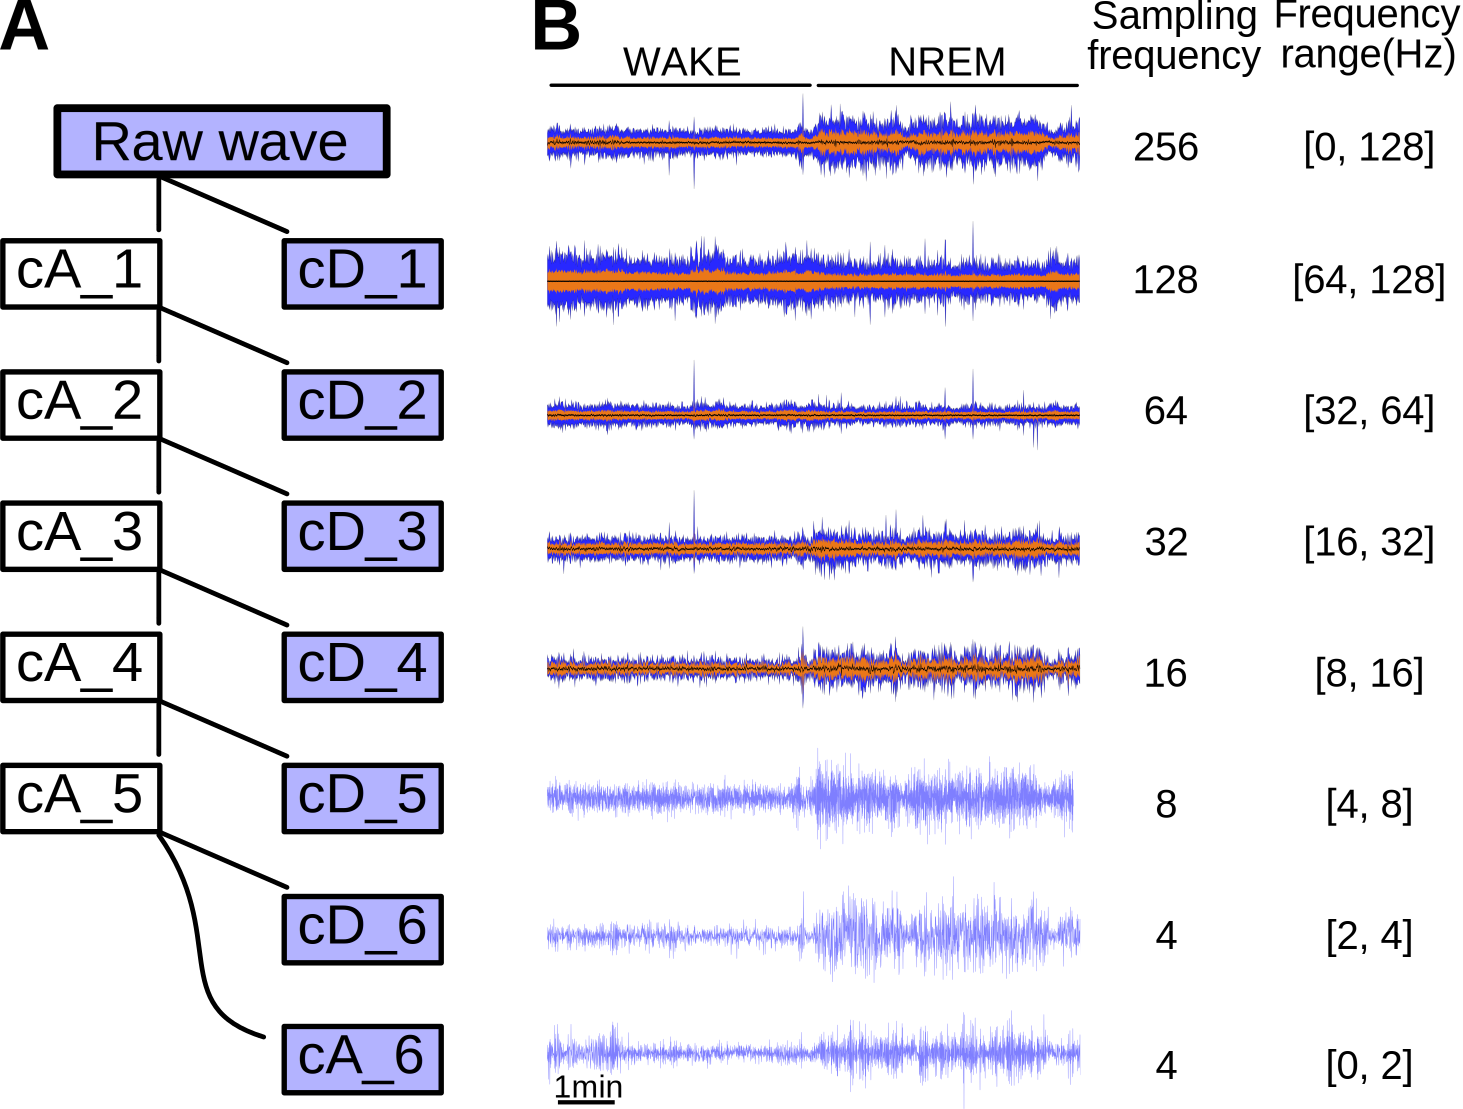
\includegraphics[width=0.95\textwidth]{figures/dwd.pdf}
  \caption{\ctit{Discrete waveletet decomposition.}
  The initial signal is split into pairs of coefficients: A and D. They capture the low ($[0, f_s/2]$), and high $[f_s/2, f_s]$ frequency information, respectively.
  Discrete wavelet transform is applied iteratively on subsequent A coefficients. In this example, decomposition is performed up to the sixth level.
  Ten minutes representing the \gls{eeg} of a transition between a wake and a slow wave sleep(NREM) are shown for the raw wave and each of the coefficients that are kept for feature extraction(blue rectangles). 
  Later, each of the eigth time series is segmented into five second epochs, and features are exhaustively computed for all wavelet coefficients as well as the raw signal.
  In this figure, the five first signals are too dense to be displayed in a naive fashion. Instead, only local range(blue), inter-quantile range (orange) and median (black line) are represented.
  \label{fig:dwd}
  }
           
\end{figure}



Importantly, discrete wavelet decomposition was applied \emph{a priory} to the whole signals.
This contrasts with applying decomposition to each epoch \citationneeded{}.
The latter method results in edge effects which would typically need to be attenuated by convolving every epoch with a window function (\eg{} Hamming window).
The maximum decomposition levels for the \gls{eeg} and \gls{emg} signals were six and four, respectively.
Daubechies wavelet, with four vanishing moments (``db4'') was used.

Discrete wavelet decomposition generated seven and five additional time series for \gls{eeg} and \gls{emg}, respectively.
Time series generated from wavelet decomposition (\ie{} coefficients) contain information relative to exclusive frequency sub-bands.
For all 14 time series, a list of 16 features (see table~\ref{tab:features}) was computed in each subsequent non-overlapping five seconds epochs.
Thus, resulting in a total of $p=192$ variables. For each recording ($\simeq 24h$) there were approximately $17000$ epochs.
Some combinations of variables and signals were however incalculable.
These were therefore removed; resulting in an actual number of variables $p=164$.



\begin {table}[!h]
\begin{center}
\caption{\ctit{List of features.}
For clarity, features were classified in four functionnal families.
16 scalar features, in four families, are computed for each epoch.
Since all features are computed for all wavelet coefficients and raw signals (\gls{eeg} and \gls{emg}), a total of 
$16 \times (1+7 + 1 + 3) = 192$ features are generated every five secon of recording.
The mathematical detail of the algorithms is provided in the documentation of \pr{} (see appendix).
\label{tab:features}}

\small
\begin{tabular}{|c|c|}
  \hline
  Feature family & features\\
 \hline
 \hline
  Power & \specialcell{\texttt{mean}, \texttt{sd}, \texttt{skewness}, \texttt{kurtosis}\\\texttt{median}, \texttt{min}, \texttt{max}}\\
  \hline
  Hjorth & \texttt{morbidity}, \texttt{complexity}\\
  \hline
  Fractal & \texttt{Petrosian} and \texttt{Higuchi} fractal dimensions\\
  \hline
  Entropy & \specialcell{\texttt{SVD} and \texttt{Fisher} entropy.\\\texttt{Sample entropy} with $m=2$, and $ r \in \{ 0.2, 1.0, 1.5\}$}\\
 \hline



\end{tabular}
\end{center}
\end{table}



As part of this project, a new \py{} package, \pr{}, was developed in order to efficiently
calculate features on heterogeneous time series.
Its complete documentation provided in the appendix of the document herein.

\subsection{Addition of temporal features}
In order to integrate temporal information, new variables, depending on past, and future values of predictors, were added for each epochs.
Given a vector $\mathbf{X_t}$ of feature at time $t$,
A first strategy was to define a new vector of feature $\mathbf{{X'}_t}$ as
\begin{equation}
\mathbf{{X'}_t} = \{\mathbf{X_{t-\tau}}, ..., \mathbf{X_t}, ..., \mathbf{X_{t+\tau}}\}
\label{eq:tau}
\end{equation}
with $\tau \in \mathbb{N}$.

Another strategy was to add features representing the local average $\mathbf{W^n_t}$ of each variable over several rectangular windows of sizes $n$.
\begin{equation}
\mathbf{{X'}_t} = \{W^{n_1}_t, W^{n_2}_t, ...\}
\label{eq:window}
\end{equation}
where
\[
\mathbf{W^n_t} = \frac{1}{2n+1} \sum_{i = t-n}^{t+n}{X_i}
\]
and $n$ is a set of odd integers representing window sizes (\eg $\{1,3,7,15\}$).



\subsection{Stratified Cross Validation}
Generally, success of classification of vigilance stages is assessed by cross-validation.
In many studies\citationneeded{}, it is implied that cross-validation was performed by making $k$ random training subsets
of the whole data and assessing the model fitted on the remaining subsets (\ie{} k-fold cross-validation). 
In this context, since features are calculated for every epoch
Therefore, epochs are the statistical individuals.

When working with dense time series (or, for instance, spatial data), it can be suspected that within a statistical block (group),
both features and response variables are very correlated with neighbouring data points.
For instance, the features and label at $t_n$ are expected to be largely similar to the features, and labels at $t_{n+1}$ and $t_{n-1}$.
In statistical terms, $t_{n+1}$ is not independent of $t_{n}$.

If the training sets are drawn completely at random, from a dataset containing multiple long recordings,
the underlying time series would only be made marginally sparser, and the data points missing from
a time series could simply be inferred from the neighbouring points which remain in the training set.
This temporal pseudo-replication may result in model overfitting and give the false impression 
that a model has a very strong predictive power.

The goal of cross-validation is to assess how well a predictive model would perform on \emph{new data}.
This study, and most similar studies, aims at providing a tool to automatically annotate \emph{new recordings}.
Therefore, it is fairer to perform \emph{stratified cross-validation}, using the different recordings as the stratum levels.
In this study, all cross-validation were performed by training the model with epochs originating from all but one recordings,
and testing it on the recording kept out. This was repeated by successively leaving each recording out.

As shown in figure~\ref{fig:sleep_description}, the prevalence of different states is not balanced. Noticeably, \gls{rem} sleep represents only $10\%$ of all epochs.
This implies that $90\%$ accuracy could be achieved even if all \gls{rem} epoch were misclassified.
For the same reason, the importance of the variables contributing to segregate the minority class (\gls{rem}) with other classes could be underestimated.
Therefore, for variable elimination (fig.~\ref{fig:variable_elimination}) and for defining new variables (fig.~\ref{fig:temporal_integration}),
balanced sub-sampled testing sets (750 epochs of each class) were used.

\subsection{Random forests}
Unless specified otherwise, random forests \citationneeded{} were trained with balanced samples of 1000 epochs per class.
Whilst this negates the prior knowledge of the state prevalences, this sampling strategy 
inflates importance of variables that are important to segregate minority from majority classes.
In order to select variables and define new features, forests with 50 classification trees were built. 
100 trees were used otherwise.
Increasing the sample size and number of trees did not seem to improve perfomance.
The number of variable drawn for each split, $mtry$, was set to the default value  for classification problems $\sqrt{p}$.
All random forest analysis was implemented in \texttt{R}\citationneeded{} statistical software, using the package \texttt{randomForest}.

In order to enrich every prediction with an associated confidence level, a probabilistic interpretation of random forest was adopted\citationneeded{}.
Then, to produce an overall summary value of confidence, an entropy based metric $c$ was defined as:
\begin{equation}
%~ \[
c = 1 + \frac{1}{log_2(k)}\sum{v_i  log_2(v_i)}
%~ \]
\label{eq:entropy}
\end{equation}
where $v_i$ is the proportion of votes for the class $i$, and $k$ is the number of classes. This definition has the properties 
\[
c \in [0;1]
\]
\[
v_1 = v_2 = ... = v_k \rightarrow c = 0
\]
\[
v_i = 1 \rightarrow c = 1 , \forall i
\]




\subsection{Performance assessments}
Comparisons of runtime between \pr{} and \pyeeg{} were performed by measuring the average (between 2 and 100 run, depending on the algorithm) runtime of algorithms on six
normally distributed ($\mathcal{N}(\mu=0,\sigma=1)$) random time series (\ie white noise) of size $n$,
with $n$ between $256 \times{} 5$ and $256 \times{} 30$.
This was repeated five times for each time series.
For computing  Higuchi fractal dimension, $k_{max}$ was set to $2^3$.
For both approximate entropy and sample entropy, the embedding dimension $m$ was set to $2$, and the distance threshold, $r$, to $1.5$.
For fisher information, the embedding dimension and the delay, $\tau$ were set to $3$ and $2$, respectively.
Finally, spectral entropy was computed for the frequency bands bounded by $\{0, 2^0, 2^1, ..., 2^6\}$Hz, with $f_s = 256.0$.
Benchmarks were generated using \texttt{CPython 2.7.8} on \texttt{GNU/Linux} operating stystem with a 3.40GHz intel i7-3770 CPU.

\subsection{Statistical analysis}
In order to test significance in the difference of performance between \pr{} and \pyeeg{} (table~\ref{tab:benchmark}),
linear models were fitted on the log-transformed runtime for each algorithm. 
t-tests on the effect of the implementation (\ie{} whether \pr{} or \pyeeg{} was used) on the intercept at $x=1280$, were used to compute $p-values$ at $n=1280$.
Significance levels for the differences in scaling were obtained through t-tests on the interaction between $n$ and the implementation.


In order to assess the significance of the effect of the addition of temporal variables on the cross-validation
error (fig.~\ref{fig:temporal_integration}), repreated t-tests were performed.
Bonferronni correction was applied.

In order to determine whether state prevalences were different between predicted and ground truth time series (fig.~\ref{fig:struct_assess}A),
beta regression \citationneeded{} was fitted. 
Then, interactions between state and method (\ie{} prediction vs. ground truth) were tested with a z-test.

In order to determine the effect of prediction on the number of episodes of each state (fig.~\ref{fig:struct_assess}B),
Poisson generalised linear linear mixed model\citationneeded{}, using recordings (\ie{} animals) as a random effect, was fitted. 
Then, interaction between state and method were tested with a t-test.

Finall, in order to determine the effect of prediction on the average duration of episodes of each state (fig.~\ref{fig:struct_assess}B),
linear linear mixed model\citationneeded{} on log-transformed duration, using recordings (\ie{} animals) as a random effect, was fitted. 
Then, interaction between state and method were tested with a t-test.

(fig.~\ref{fig:struct_assess}A)




\newpage{}
\section{Results} \label{results}

lorem ipsum ...
\subsection{\texttt{Python} package}
Speed Improvement. correction of math formulae.

\begin {table}[!h]
\begin{center}
\caption{\ctit{Performance improvements over \texttt{PyEEG}.}
In order to improve performance, modifications of the algorithms implemented in \texttt{PyEEG} were carried out.
This table compares how long, on average, each algorithm would take, for a random sequence of length $1280$ (\ie{} $5s$ at $256$Hz).
It also represents how many added points would lead to a tenfold runtime increase.
For the tested range ($n \in [1280;7680] $), all algorithms add approximately an
exponential time complexity ($10^{O(n)}$, $R^2 > 0.95$, for all).
Several mathematical inconsistencies were also discovered and corrected. 
The rightmost column (\textbf{\textdagger}) indicates whether the original implementation was
corrected in order to match mathematical definition. Each alteration is mathematically justified in the section \texttt{pyrem.univariate} of the \pr{} documentation (see appendix).
\textbf{(-)}: indicates a worse performance of \pr{} over \pyeeg{}.
Significance levels: $^{***}$, $p-value < 10^{-3}$; $^{**}$, $p-value < 10^{-2}$, see Material and Methods for detail about statistical analysis.
\label{tab:benchmark}
}
\footnotesize
\begin{tabular}{|c|c|c|c|c|c|c|}
  \hline
  &  & \multicolumn{2}{|c|}{\texttt{PyEEG}} & \multicolumn{2}{|c|}{\pr} & \\
 \hline
 \hline
 
  algorithm & function & \specialcell{$t$(ms) for \\$n = 1280$} & \specialcell{$n$ for $\times 10$\\increase} & \specialcell{$t$(ms) for \\$n = 1280$} & \specialcell{$n$ for $\times 10$\\ increase} & fix\textsuperscript{\textdagger}\\
 
  \hline
  \hline
\specialcell{Approximate\\Entropy} & \texttt{ap\_ent} &                                     9970 & 4288 & $487^{***}$ & $3478^{***}(-)$ & No\\
\hline
Fisher Information & \texttt{fisher\_info} &                                 3.24 & 8673 & $0.121^{***}$ & $12427^{***}$ & No\\
\hline
\specialcell{Higuchi\\Fractal Dimension} & \texttt{hfd} &                     11.7 & 8833 & $1.39^{***}$ & $28329^{***}$ & Yes\\
\hline
Hjorth parameters & \texttt{hjorth} &                                         5.14 & 8633 & $0.088^{***}$ & $36354^{***}$ & Yes\\
\hline
\specialcell{Petrosian\\Fractal Dimension} & \texttt{pfd} &                 2.66 & 8606 & 2.65 & 8579 & Yes\\
\hline
Sample Entropy & \texttt{samp\_ent} &                                         8305 & 4276 & $188^{***}$ & $5483^{***}(-)$ & No\\
\hline
Spectral Entropy & \texttt{spectral\_entropy} &                                 0.309 & 11459 & $0.227^{***}$ & $22133^{***}$ & Yes\\
\hline
\specialcell[l]{Singular Value \\Decomposition\\ entropy} & \texttt{svd\_ent} &     3.25 & 8663 & $0.113^{***}$ & $11774^{**}$ & Yes\\
 \hline
\end{tabular}
\end{center}
\end{table}

Interface imporvement (see package doc)

Visualisation (explain why it is important)

\subsection{DWT, feature extraction strategy}
Explain typycal approach, and why using DWT and then epoching is advantageaous while remaing fast.

\subsection{Important features}
$n$ is large, reducing $p$ could make the analysis faster. computing each $p$ feature is slow.
variable importance can be used to select a subset of informative variable.

20ish variable are good enough.

The analysis can be rendered faster
\subsection{Including temporal information}
Using features at $\mathbf{Z} = \{\mathbf{X_{t-\tau}}, ..., \mathbf{X_{t}}, ..., \mathbf{X_{t+\tau}}\}$ provide a significant improvement over $\mathbf{Z} = \mathbf{X_{t}}$.

It does not seem adventageous to use $\tau > 3$.
\subsection{Deeper assesment}

\newpage{}
\section{Discussion} \label{discussion}

\subsection{python package} 
Clear improvement over existing software.

Faster, less math mistake

more features.

Independant from sleep, so can be used fort other stuff

why sample entropy and ap entropy do not as well...

julia link

public relase of this package


\subsection{Originality of feature extraction} 
Feature extraction is more exhaustive.
it turns out that some wavelet specific features were  important predictor
include temporal features.
why is that controvertial => sleep is assumed to be consistant

\subsection{Using random forest} 

* Variable importance (investigation ++)

* white box

* General classifier, so we can use the exact same data and something like ANN

* Efficient

* natural inclusion of non linearity, which is expected when we get more data

\subsection{Originality of crossvalidation} 

Very conservative


\TODO{make a "movement" label}


\TODO{More animals would be better}


\newpage{}
%~ \bibliography{report.bib}{}
%~ \bibliographystyle{ieeetr}

%~ \newpage{}
%~ \begin{appendices}
%~ \section{Documentation}
%~ \end{appendices}
   
\end{document}
